\documentclass[11pt,a4paper]{article}
\usepackage[T1]{fontenc}
\usepackage[utf8]{inputenc}
\usepackage{lmodern}
\usepackage{textcomp}
\usepackage[left=1.8cm,right=1.8cm,top=2.3cm,bottom=2.2cm,headheight=14pt,headsep=8pt]{geometry}
\usepackage{multicol}
\usepackage{xcolor}
\usepackage{fancyhdr}
\usepackage{graphicx}
\usepackage{array}
\usepackage{amsmath,amssymb}
\usepackage{setspace}
\usepackage{longtable}
\graphicspath{{../}}
\definecolor{ygreen}{RGB}{46,139,87}
\renewcommand{\normalsize}{\fontsize{10.9}{13.4}\selectfont}
\renewcommand{\familydefault}{\rmdefault}
\setlength{\parindent}{0pt}
\setlength{\columnsep}{0.8cm}
\setlength{\columnseprule}{0.4pt}
\setlength{\multicolsep}{3pt plus 1pt minus 1pt}
\renewcommand{\textsubscript}[1]{\ensuremath{_{\text{\fontsize{8}{8}\selectfont #1}}}}
\renewcommand{\textsuperscript}[1]{\ensuremath{^{\text{\fontsize{8}{8}\selectfont #1}}}}
\newcommand{\qn}[1]{\textbf{\fontsize{11.5}{13}\selectfont #1}}
\newcommand{\qsep}{\par\vspace{1pt}\noindent\rule{0pt}{0.4pt}\par\vspace{5pt}}
\newcommand{\fwrule}{\par\vspace{5pt}\noindent\rule{\linewidth}{1.4pt}\par\vspace{7pt}}
\newsavebox{\fitb}
\newcommand{\fitbox}[1]{\sbox{\fitb}{#1}\ifdim\wd\fitb>\linewidth\resizebox{\linewidth}{!}{\usebox{\fitb}}\else\usebox{\fitb}\fi}
\newcommand{\diqqat}[1]{\par\smallskip\noindent\textbf{Diqqat!} #1\par\medskip}
\newcommand{\javob}{\par\smallskip\noindent\textbf{Javob:} \rule[-2pt]{7.5cm}{0.4pt}\par\smallskip\noindent\textbf{Diqqat!} Javobingizni javoblar varaqasiga ko`chirib yozing.\par\medskip}
\pagestyle{fancy}
\fancyhf{}
\renewcommand{\headrulewidth}{0.4pt}
\fancyhead[L]{\textit{Milliy sertifikat 2026. Kimyo}}
\fancyhead[R]{9-variant}
\fancyfoot[L]{\fontsize{8}{9}\selectfont \textcopyright{} Colba maktabi, 2026}
\fancyfoot[C]{\thepage}
\fancypagestyle{first}{\fancyhf{}\renewcommand{\headrulewidth}{0pt}\fancyfoot[L]{\fontsize{8}{9}\selectfont \textcopyright{} Colba maktabi, 2026}\fancyfoot[C]{\thepage}}
\begin{document}
\normalsize
\thispagestyle{first}
\noindent\fcolorbox{ygreen}{white}{\parbox{\dimexpr\linewidth-2\fboxsep-2\fboxrule\relax}{%
\textbf{\fontsize{13}{15}\selectfont Nazorat testi}\ \textit{\fontsize{10}{12}\selectfont $\cdot$ Aralash test $\cdot$ 9-variant}\hfill
\begin{tabular}[t]{@{}r@{}}\textit{Milliy sertifikat 2026. Kimyo}\\ \textbf{\textit{\fontsize{8}{9}\selectfont Vaqt:}} \textit{\fontsize{10}{12}\selectfont 180 daqiqa}\end{tabular}}}
\par\medskip
\noindent\textit{Davriy jadvaldan foydalanish mumkin.}
\par\medskip
\begin{multicols}{2}
\noindent\qn{1.} A + B $\rightleftarrows$ C reaksiyada moddalar konsentratsiyalarining vaqt bo`yicha o`zgarishi grafikda ko`rsatilgan.
\begin{center}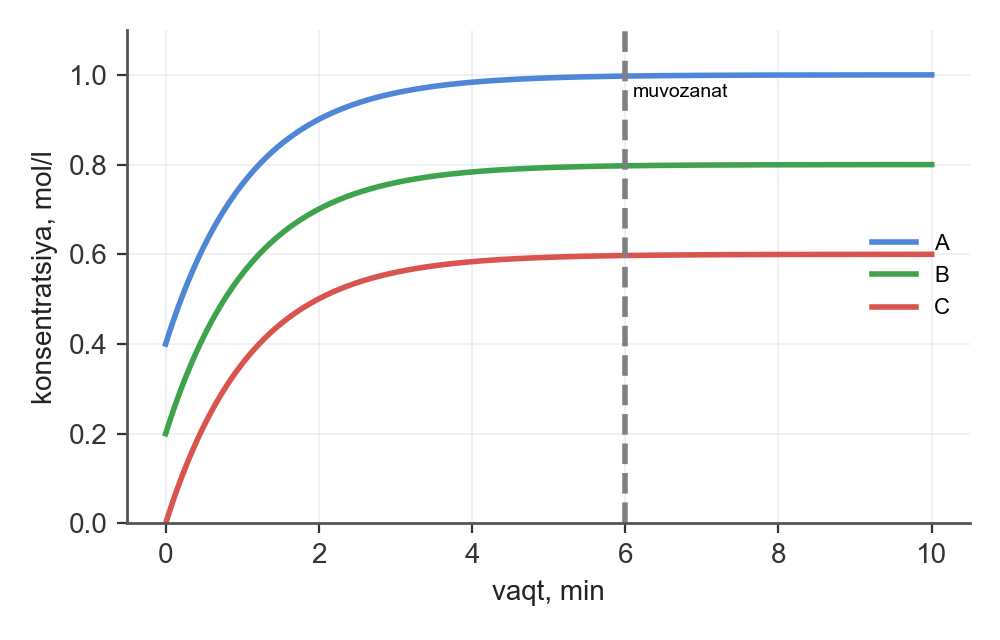
\includegraphics[width=0.86\linewidth]{rasmlar/gen/conc_v09_0.png}\end{center}
Grafikdan foydalanib, muvozanat \textbf{konstantasini (K) aniqlang.}

\noindent A)~\textsl{15} \hfill B)~\textsl{7,5} \hfill C)~\textsl{3,75} \hfill D)~\textsl{1}\par
\qsep
\noindent\qn{2.} Quyidagi zarrachalardan qaysilari neon atomi bilan izoelektron? 1) Al\textsuperscript{3+}; 2) Cl\textsuperscript{$-$}; 3) S\textsuperscript{2$-$}; 4) F\textsuperscript{$-$}

\noindent A)~\textsl{2, 3, 4} \hfill B)~\textsl{1, 2} \hfill C)~\textsl{1, 4} \hfill D)~\textsl{2, 4}\par
\qsep
\noindent\qn{3.} N\textsubscript{2} + 3H\textsubscript{2} $\rightleftarrows$ 2NH\textsubscript{3} reaksiyasi 2 l hajmli idishda o`tkazildi. Ma'lumotlar jadvalda berilgan:
\begin{center}
\renewcommand{\arraystretch}{1.15}
\fitbox{\begin{tabular}{|c|c|c|c|}\hline
\textbf{Modda} & \textbf{N\textsubscript{2}} & \textbf{H\textsubscript{2}} & \textbf{NH\textsubscript{3}} \\ \hline
Boshlang`ich, mol & 4 & 6 & 0 \\ \hline
Muvozanatda, mol & --- & --- & 2 \\ \hline
\end{tabular}}
\end{center}
N\textsubscript{2} ning necha foizi reaksiyaga \textbf{kirishganini aniqlang.}

\noindent A)~\textsl{12,5} \hfill B)~\textsl{25} \hfill C)~\textsl{37,5} \hfill D)~\textsl{75}\par
\qsep
\noindent\qn{4.} Quyidagi tuzlarning qaysilari suvli eritmasi ishqoriy muhitga ega? 1) K\textsubscript{3}PO\textsubscript{4}; 2) ZnCl\textsubscript{2}; 3) K\textsubscript{2}SO\textsubscript{4}; 4) NH\textsubscript{4}Cl

\noindent A)~\textsl{1} \hfill B)~\textsl{2, 3} \hfill C)~\textsl{3} \hfill D)~\textsl{3, 4}\par
\qsep
\noindent\qn{5.} Gazlar aralashmasi tarkibi jadvalda berilgan (n.sh.):
\begin{center}
\renewcommand{\arraystretch}{1.15}
\fitbox{\begin{tabular}{|c|c|}\hline
\textbf{Gaz} & \textbf{Hajmi, l} \\ \hline
He & 1 \\ \hline
N\textsubscript{2} & 1 \\ \hline
SO\textsubscript{2} & 2 \\ \hline
\end{tabular}}
\end{center}
Aralashmaning havoga nisbatan \textbf{zichligini aniqlang} (M(havo) = 29 g/mol).

\noindent A)~\textsl{2,76} \hfill B)~\textsl{0,69} \hfill C)~\textsl{40} \hfill D)~\textsl{1,38}\par
\qsep
\noindent\qn{6.} Reaksiya tezligining harorat koeffitsiyenti $\gamma$ = 4. 20 \textdegree{}C da reaksiya 32 minutda tugasa, 40 \textdegree{}C da necha sekundda tugaydi?

\noindent A)~\textsl{30720} \hfill B)~\textsl{480} \hfill C)~\textsl{2} \hfill D)~\textsl{120}\par
\qsep
\noindent\qn{7.} 1 M HCl eritmasining normal \textbf{konsentratsiyasini (n) aniqlang.}

\noindent A)~\textsl{2} \hfill B)~\textsl{0,5} \hfill C)~\textsl{1} \hfill D)~\textsl{1,5}\par
\qsep
\noindent\qn{8.} NaCl eritmasi inert elektrodlar yordamida 10 A tok kuchi bilan 965 s elektroliz qilindi. Anodda ajralgan Cl\textsubscript{2} hajmi (l, n.sh.) \textbf{ni toping.}

\noindent A)~\textsl{2,24} \hfill B)~\textsl{1,12} \hfill C)~\textsl{0,56} \hfill D)~\textsl{0,112}\par
\qsep
\noindent\qn{9.} H\textsubscript{2} + I\textsubscript{2} $\rightleftarrows$ 2HI reaksiyada muvozanat qaror topganda [H\textsubscript{2}] = 1, [I\textsubscript{2}] = 2, [HI] = 4 mol/l bo`ldi. I\textsubscript{2} ning boshlang`ich \textbf{konsentratsiyasini (mol/l) aniqlang.}

\noindent A)~\textsl{4} \hfill B)~\textsl{2} \hfill C)~\textsl{6} \hfill D)~\textsl{8}\par
\qsep
\noindent\qn{10.} Faqat oksidlovchi bo`la oladigan \textbf{ionlarni aniqlang}: 1) I\textsuperscript{$-$}; 2) Cl\textsuperscript{$-$}; 3) K\textsuperscript{+}; 4) Na\textsuperscript{+}

\noindent A)~\textsl{1} \hfill B)~\textsl{1, 2, 4} \hfill C)~\textsl{2, 4} \hfill D)~\textsl{3, 4}\par
\qsep
\noindent\qn{11.} CuCl\textsubscript{2} ning suvli eritmasi inert elektrodlar bilan elektroliz qilinganda qaysi moddalar ajraladi?

\noindent\begin{tabular}{@{}p{0.47\linewidth}@{}p{0.47\linewidth}@{}}
A)~\textsl{Cu va O\textsubscript{2}} & B)~\textsl{Cu va Cl\textsubscript{2}} \\
C)~\textsl{Zn, H\textsubscript{2} va O\textsubscript{2}} & D)~\textsl{Ag va O\textsubscript{2}} \\
\end{tabular}\par
\qsep
\noindent\qn{12.} 4,6 g Na va 3,55 g Cl\textsubscript{2} aralashtirilib, reaksiya o`tkazildi (2Na + Cl\textsubscript{2} $\to$ 2NaCl). Hosil bo`lgan NaCl \textbf{massasini (g) aniqlang.}

\noindent A)~\textsl{5,85} \hfill B)~\textsl{11,7} \hfill C)~\textsl{2,93} \hfill D)~\textsl{8,78}\par
\qsep
\noindent\qn{13.} 18,25 g HCl 500 g suvda eritildi. Eritmaning molyal \textbf{konsentratsiyasini (mol/kg) aniqlang.}

\noindent A)~\textsl{0,96} \hfill B)~\textsl{0} \hfill C)~\textsl{2} \hfill D)~\textsl{1}\par
\qsep
\noindent\qn{14.} Reaksiya tenglamasi: ZnO + 2HCl $\to$ ZnCl\textsubscript{2} + H\textsubscript{2}O. Reaksiyaga tarkibida 20\% aralashma bo`lgan 20,25 g namuna (asosiy modda ZnO) kirishdi. HCl \textbf{hajmini (l, n.sh.) hisoblang.}

\noindent A)~\textsl{2,24} \hfill B)~\textsl{17,92} \hfill C)~\textsl{8,96} \hfill D)~\textsl{4,48}\par
\qsep
\noindent\qn{15.} Mg(HCO\textsubscript{3})\textsubscript{2} $\to$ MgCO\textsubscript{3} + CO\textsubscript{2} + H\textsubscript{2}O reaksiyasida 146 g Mg(HCO\textsubscript{3})\textsubscript{2} ishtirok etdi. MgCO\textsubscript{3} \textbf{massasini (g) toping.}

\noindent A)~\textsl{168} \hfill B)~\textsl{42} \hfill C)~\textsl{84} \hfill D)~\textsl{126}\par
\qsep
\noindent\qn{16.} Reaksiya tenglamasi: N\textsubscript{2}O\textsubscript{5} + H\textsubscript{2}O $\to$ 2HNO\textsubscript{3}. Reaksiyaga tarkibida 10\% aralashma bo`lgan 12 g namuna (asosiy modda N\textsubscript{2}O\textsubscript{5}) kirishdi. HNO\textsubscript{3} \textbf{massasini (g) hisoblang.}

\noindent A)~\textsl{3,15} \hfill B)~\textsl{25,2} \hfill C)~\textsl{12,6} \hfill D)~\textsl{6,3}\par
\qsep
\noindent\qn{17.} P $\to$ ? $\to$ ? $\to$ ? o`zgarishlar zanjirida (reagentlar: O\textsubscript{2}, H\textsubscript{2}O, KOH) 3-bosqichda hosil bo`ladigan modda \textbf{formulasini toping.}

\noindent A)~\textsl{SO\textsubscript{2}} \hfill B)~\textsl{Na\textsubscript{2}O} \hfill C)~\textsl{K\textsubscript{3}PO\textsubscript{4}} \hfill D)~\textsl{NaOH}\par
\qsep
\noindent\qn{18.} NH\textsubscript{3} + H\textsubscript{3}PO\textsubscript{4} $\to$ NH\textsubscript{4}H\textsubscript{2}PO\textsubscript{4} jarayoni uchun 98 g H\textsubscript{3}PO\textsubscript{4} olingan (unum 60\%). NH\textsubscript{4}H\textsubscript{2}PO\textsubscript{4} \textbf{massasini (g) aniqlang.}

\noindent A)~\textsl{115} \hfill B)~\textsl{138} \hfill C)~\textsl{69} \hfill D)~\textsl{34,5}\par
\qsep
\noindent\qn{19.} NH\textsubscript{4}NO\textsubscript{3} qizdirilganda qanday moddalar hosil bo`ladi?

\noindent\begin{tabular}{@{}p{0.47\linewidth}@{}p{0.47\linewidth}@{}}
A)~\textsl{Ag, NO\textsubscript{2} va O\textsubscript{2}} & B)~\textsl{KNO\textsubscript{2} va O\textsubscript{2}} \\
C)~\textsl{CuO, NO\textsubscript{2} va O\textsubscript{2}} & D)~\textsl{N\textsubscript{2}O va H\textsubscript{2}O} \\
\end{tabular}\par
\qsep
\noindent\qn{20.} CH\textsubscript{4} + Cl\textsubscript{2} $\to$ CH\textsubscript{3}Cl + HCl jarayoni uchun 4,48 l (n.sh.) CH\textsubscript{4} olingan. CH\textsubscript{3}Cl \textbf{miqdorini (mol) aniqlang.}

\noindent A)~\textsl{0,4} \hfill B)~\textsl{0,1} \hfill C)~\textsl{0,3} \hfill D)~\textsl{0,2}\par
\qsep
\noindent\qn{21.} Alken, alkadiyen va alkinlar haqida qaysi fikrlar to`g`ri? 1) Alkinlar uchun umumiy formula CnH\textsubscript{2}n+2; 2) Asetilen Ag\textsubscript{2}O ning ammiakli eritmasi bilan cho`kma beradi (butin-2 beradi); 3) Etilen bromli suvni rangsizlantiradi; 4) Alkenlarda $\pi$-bog` yo`q

\noindent A)~\textsl{2, 3} \hfill B)~\textsl{3} \hfill C)~\textsl{1, 4} \hfill D)~\textsl{1, 3}\par
\qsep
\noindent\qn{22.} Rasmda siklik uglevodorodning tuzilish formulasi berilgan.
\begin{center}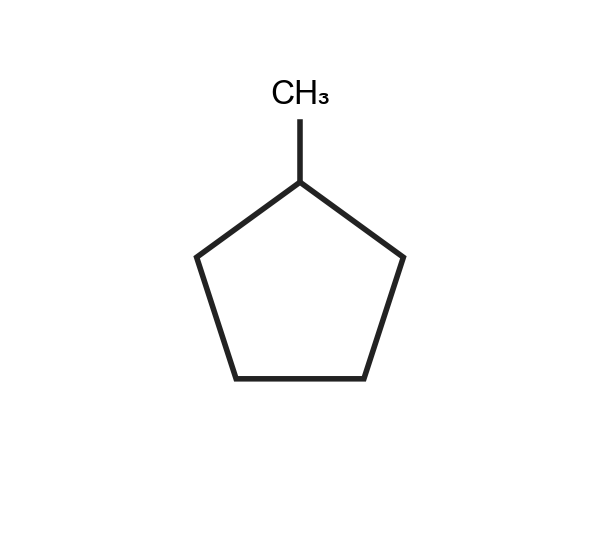
\includegraphics[width=0.86\linewidth]{rasmlar/gen/rn_873219.png}\end{center}
Birikmaning \textbf{nomini toping.}

\noindent\begin{tabular}{@{}p{0.47\linewidth}@{}p{0.47\linewidth}@{}}
A)~\textsl{1,2-dimetilsiklogeksan} & B)~\textsl{metilsiklopropan} \\
C)~\textsl{1,2-dimetilsiklopentan} & D)~\textsl{metilsiklopentan} \\
\end{tabular}\par
\qsep
\noindent\qn{23.} Spirt va fenollar haqida qaysi fikrlar to`g`ri? 1) Fenol FeCl\textsubscript{3} bilan binafsha rang beradi; 2) Glitserin Cu(OH)\textsubscript{2} bilan ko`k kompleks hosil qiladi; 3) Fenol Cu(OH)\textsubscript{2} ni eritib ko`k kompleks hosil qiladi; 4) Uchlamchi spirtlar oson oksidlanadi

\noindent A)~\textsl{4} \hfill B)~\textsl{1, 2} \hfill C)~\textsl{3} \hfill D)~\textsl{1, 2, 4}\par
\qsep
\noindent\qn{24.} 18 g glyukoza Ag\textsubscript{2}O ning ammiakli eritmasi bilan to`liq oksidlanganda hosil bo`lgan kumush \textbf{massasini (g) aniqlang.}

\noindent A)~\textsl{21,6} \hfill B)~\textsl{10,8} \hfill C)~\textsl{43,2} \hfill D)~\textsl{18}\par
\qsep
\noindent\qn{25.} Karbon kislotalar haqida qaysi fikrlar to`g`ri? 1) Sirka kislota karbonatlar bilan CO\textsubscript{2} ajratadi; 2) Sirka angidrid ikki molekula sirka kislotadan suv chiqib hosil bo`ladi; 3) Benzoy kislota Na\textsubscript{2}CO\textsubscript{3} bilan reaksiyaga kirishmaydi; 4) Olein kislota Br\textsubscript{2} ni biriktiradi

\noindent A)~\textsl{1, 2, 4} \hfill B)~\textsl{1, 3} \hfill C)~\textsl{2, 3, 4} \hfill D)~\textsl{2, 4}\par
\qsep
\noindent\qn{26.} Murakkab efirlar va yog`lar haqida qaysi fikrlar to`g`ri? 1) Suyuq yog`lar to`yinmagan kislotalardan hosil bo`lgan; 2) Yog`lar glitserin va yuqori yog` kislotalarning murakkab efirlari; 3) Efirlanish reaksiyasi qaytmas; 4) Sovun --- yuqori yog` kislotalarning natriyli tuzi

\noindent A)~\textsl{1, 4} \hfill B)~\textsl{1, 2, 4} \hfill C)~\textsl{1, 3, 4} \hfill D)~\textsl{1, 3}\par
\qsep
\noindent\qn{27.} Uglevodlar haqida qaysi fikrlar to`g`ri? 1) Kraxmal yod bilan ko`k rang beradi; 2) Selluloza $\beta$-glyukoza qoldiqlaridan iborat; 3) Glyukoza gidrolizlanadi; 4) Glyukoza "kumush ko`zgu" reaksiyasini beradi

\noindent A)~\textsl{1, 3, 4} \hfill B)~\textsl{2, 3} \hfill C)~\textsl{1, 2, 4} \hfill D)~\textsl{1, 2, 3}\par
\qsep
\noindent\qn{28.} 15 g glitsin HCl bilan reaksiyaga kirishganda hosil bo`lgan tuz \textbf{massasini (g) aniqlang.}

\noindent A)~\textsl{22,3} \hfill B)~\textsl{15} \hfill C)~\textsl{7,3} \hfill D)~\textsl{44,6}\par
\qsep
\noindent\qn{29.} 5,6 g C\textsubscript{2}H\textsubscript{4} dan quyidagi ikki bosqichda C\textsubscript{2}H\textsubscript{5}OH olinadi: 1) C\textsubscript{2}H\textsubscript{4} + HCl $\to$ C\textsubscript{2}H\textsubscript{5}Cl (unum 80\%); 2) C\textsubscript{2}H\textsubscript{5}Cl + KOH $\to$ C\textsubscript{2}H\textsubscript{5}OH + KCl (unum 75\%). Oxirgi mahsulot C\textsubscript{2}H\textsubscript{5}OH ning \textbf{massasini (g) toping.}

\noindent A)~\textsl{6,9} \hfill B)~\textsl{5,52} \hfill C)~\textsl{7,36} \hfill D)~\textsl{9,2}\par
\qsep
\noindent\qn{30.} Rasmda tasvirlangan usul bilan qaysi aralashmani ajratish mumkin?
\begin{center}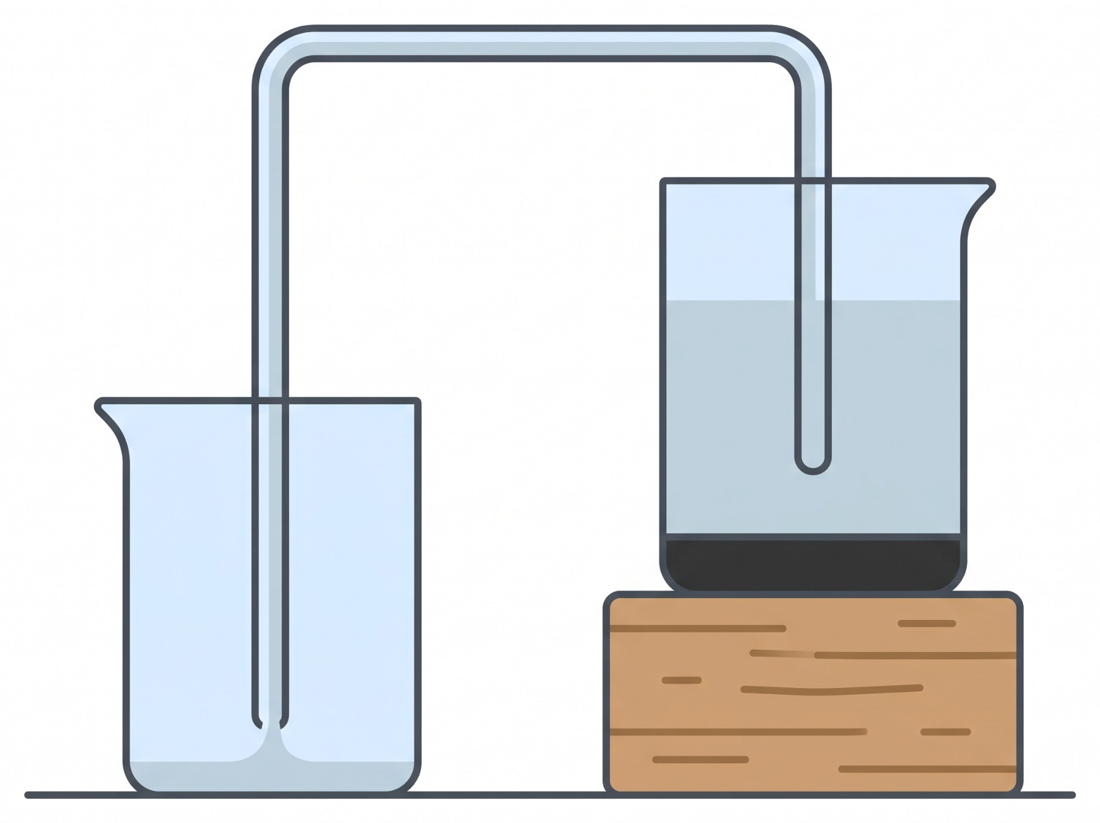
\includegraphics[width=0.86\linewidth]{rasmlar/darslik/d_tindirish.png}\end{center}
\noindent A)~\textsl{loyqa suv (suv va qum zarrachalari)}\par
\noindent B)~\textsl{suv va etanol}\par
\noindent C)~\textsl{suv va kerosin}\par
\noindent D)~\textsl{osh tuzi eritmasi}\par
\qsep
\noindent\qn{31.} Quyidagi aralashmani ajratish uchun qaysi usul mos: suv va etanol aralashmasi?
\noindent A)~\textsl{distillash (fraksiyalab haydash)}\par
\noindent B)~\textsl{ajratgich voronka}\par
\noindent C)~\textsl{bug`latish}\par
\noindent D)~\textsl{magnit yordamida ajratish (temir tortiladi)}\par
\qsep
\noindent\qn{32.} Eritmaga BaCl\textsubscript{2} qo`shilganda oq cho`kma (BaSO\textsubscript{4}), HCl da erimaydi kuzatildi. Eritmada qaysi ion bor?

\noindent\begin{tabular}{@{}p{0.47\linewidth}@{}p{0.47\linewidth}@{}}
A)~\textsl{NH\textsubscript{4}\textsuperscript{+}} & B)~\textsl{Br\textsuperscript{$-$}} \\
C)~\textsl{CO\textsubscript{3}\textsuperscript{2$-$}} & D)~\textsl{SO\textsubscript{4}\textsuperscript{2$-$}   ---} \\
\end{tabular}\par
\qsep
\end{multicols}
\medskip
\noindent\setlength{\fboxsep}{0pt}\fbox{\begin{tabular}{p{0.74\linewidth}|p{0.2\linewidth}}
\parbox[t]{0.72\linewidth}{\vspace{3pt}\textbf{Topshiriqlar (33--35) va javob variant (A--F)larini o`zaro to`g`ri moslashtiring.} NaBr va NaCl dan iborat 16,15 g aralashma suvda eritilib, mo`l AgNO\textsubscript{3} eritmasi qo`shildi; hosil bo`lgan cho`kmalarning umumiy massasi 33,15 g.
\vspace{3pt}} & \parbox[t]{0.19\linewidth}{\vspace{3pt}A~\textsl{5,15}\\[3pt]
B~\textsl{8,5}\\[3pt]
C~\textsl{10,3}\\[3pt]
D~\textsl{17}\\[3pt]
E~\textsl{340}\\[3pt]
F~\textsl{510}}\\ \hline
\parbox[t]{0.72\linewidth}{\vspace{2pt}\textbf{33. Aralashmadagi NaBr massasini (g) aniqlang.}\vspace{2pt}} & \\ \hline
\parbox[t]{0.72\linewidth}{\vspace{2pt}\textbf{34. Sarflangan 10\% li AgNO\textsubscript{3} eritmasining massasini (g) aniqlang (M(AgNO\textsubscript{3}) = 170 g/mol).}\vspace{2pt}} & \\ \hline
\parbox[t]{0.72\linewidth}{\vspace{2pt}\textbf{35. Eritmada hosil bo`lgan nitratlarning umumiy massasini (g) aniqlang.}\vspace{2pt}} & 
\end{tabular}}
\par\bigskip
\noindent\qn{36.} Cu + HNO\textsubscript{3} $\to$ Cu(NO\textsubscript{3})\textsubscript{2} + NO + H\textsubscript{2}O reaksiya tenglamasini tenglang va barcha koeffitsiyentlar \textbf{yig`indisini aniqlang.}
\javob\qsep
\noindent\qn{37.} Reaksiya 30 \textdegree{}C da 72 minutda tugaydi. $\gamma$ = 2. Harorat 20 \textdegree{}C ga oshirilib, reagentlardan birining konsentratsiyasi 2 marta oshirildi (reaksiya shu modda bo`yicha 1-tartibli). Reaksiya necha minutda tugaydi?
\javob\qsep
\noindent\qn{38.} 37,6 g Cu(NO\textsubscript{3})\textsubscript{2} qizdirilganda qisman parchalandi, qattiq qoldiq massasi 26,8 g bo`ldi. Ajralgan gazlar (n.sh.) \textbf{hajmini (l) hisoblang.}
\javob\qsep
\noindent\qn{39.} Etilen va asetilendan iborat 4,48 l (n.sh.) aralashma bromli suvdan o`tkazilganda 40 g brom yutildi. Aralashmadagi asetilenning \textbf{hajmini (l, n.sh.) toping.}
\javob\qsep
\noindent\qn{40.} Polistirol polimerining (polimerlanish darajasi 2000) 416 g namunasini olish uchun polimerlanish unumi 80\% bo`lganda qancha monomer (C\textsubscript{8}H\textsubscript{8}) kerak (g)?
\javob\qsep
\par\bigskip\begin{center}\textbf{\fontsize{13}{15}\selectfont YOZMA ISH}\end{center}
\noindent\qn{41.} \textbf{Topshiriqni bajarish jarayonida barcha reaksiya tenglamalarini yozing. Miqdoriy va arifmetik hisoblashlarni (unga asos bo`lgan usul yoki formulani ko`rsatgan holda) uzviy ketma-ketlikda bajaring.}\par\smallskip
Elementar 2SO\textsubscript{2} + O\textsubscript{2} $\to$ 2SO\textsubscript{3} reaksiyasi 30 \textdegree{}C da 162 minutda tugaydi. Reaksiyaning temperatura koeffitsiyenti $\gamma$ = 3. Boshlang`ich konsentratsiyalar [SO\textsubscript{2}] = [O\textsubscript{2}] = 0,2 mol/l bo`lganda boshlang`ich tezlik 1$\cdot$10\textsuperscript{$-$3} mol/(l$\cdot$min) ga teng.\par
\noindent 1)Reaksiya tezligi konstantasini (k) hisoblang va kinetik tenglamani yozing.\par
\noindent 2)Harorat 40 \textdegree{}C ga oshirilganda reaksiya tezligi necha marta ortadi? Reaksiyaning 40 \textdegree{}C dagi to`liq vaqtini soatda (taxminan) ham ifodalang.\par
\noindent 3)Harorat 40 \textdegree{}C ga oshirilganda reaksiya necha minutda tugaydi?\par
\noindent 4)Idish hajmi 2 marta kamaytirilsa, 30 \textdegree{}C da tezlik necha marta o`zgaradi? Idish hajmi 3 marta oshirilsa tezlik necha marta kamayadi?\par
\noindent 5)SO\textsubscript{2} ning konsentratsiyasini 3 marta oshirib, O\textsubscript{2} niki o`zgarmasa, tezlik necha marta o`zgaradi? Shuningdek harorat 30 \textdegree{}C dan 10 \textdegree{}C gacha pasaytirilsa tezlik necha marta kamayadi?\par
\diqqat{Mazkur topshiriq kengaytirilgan javobni talab etib, uning yechilish usuli va shu usul asosidagi barcha hisoblash amallari javoblar varaqasida aks etishi lozim.}\qsep
\noindent\qn{42.} Quyidagi o`zgarishlar zanjirida \textit{X}, \textit{Y}, \textit{Z} noma'lum organik moddalar:\par
\[\setlength{\fboxsep}{0pt}\text{C\textsubscript{2}H\textsubscript{5}OH}\xrightarrow{\text{CuO, t\textdegree{}}}\text{\textit{X}}\xrightarrow{\text{Ag\textsubscript{2}O, NH\textsubscript{3}}}\text{\textit{Y}}\xrightarrow{\text{Cl\textsubscript{2}, P}}\text{\textit{Z}}\xrightarrow{\text{NH\textsubscript{3}}}\text{NH\textsubscript{2}CH\textsubscript{2}COOH}\]
\noindent 1)C\textsubscript{2}H\textsubscript{5}OH $\to$ \textit{X} : reaksiya tenglamasini yozing; hosil bo`lgan moddani nomlang.\par
\noindent 2)\textit{X} $\to$ \textit{Y} : reaksiya tenglamasini yozing; hosil bo`lgan moddani nomlang.\par
\noindent 3)\textit{Y} $\to$ \textit{Z} : reaksiya tenglamasini yozing; hosil bo`lgan moddani nomlang.\par
\noindent 4)\textit{Z} $\to$ NH\textsubscript{2}CH\textsubscript{2}COOH : reaksiya tenglamasini yozing; hosil bo`lgan moddani nomlang.\par
\diqqat{Mazkur topshiriq kengaytirilgan javobni talab etib, uning yechilish usuli va shu usul asosidagi barcha hisoblash amallari javoblar varaqasida aks etishi lozim.}\qsep
\noindent\qn{43.} \textbf{Topshiriqni bajarish jarayonida barcha reaksiya tenglamalarini yozing. Miqdoriy va arifmetik hisoblashlarni (unga asos bo`lgan usul yoki formulani ko`rsatgan holda) uzviy ketma-ketlikda bajaring.}\par\smallskip
12,4 g qizil fosfor mo`l kislorodda yondirildi, hosil bo`lgan oksid suvda to`liq eritildi (ortofosfat kislota). Eritmaga 0,8 mol NaOH qo`shildi.\par
\noindent 1)Reaksiya tenglamalarini yozing. Hosil bo`lgan P\textsubscript{2}O\textsubscript{5} massasini (g) hisoblang.\par
\noindent 2)Hosil bo`lgan H\textsubscript{3}PO\textsubscript{4} massasini (g) toping. Kislotada fosforning massa ulushini (\%) ham hisoblang.\par
\noindent 3)Eritmada qanday tuz hosil bo`lganini aniqlang va uning massasini (g) hisoblang.\par
\noindent 4)Hosil bo`lgan eritmani to`liq neytrallash uchun yana qancha NaOH (g) kerak (Na\textsubscript{2}HPO\textsubscript{4} $\to$ Na\textsubscript{3}PO\textsubscript{4})?\par
\noindent 5)Hosil bo`lgan tuzning 10\% li eritmasi massasini (g) hisoblang.\par
\diqqat{Mazkur topshiriq kengaytirilgan javobni talab etib, uning yechilish usuli va shu usul asosidagi barcha hisoblash amallari javoblar varaqasida aks etishi lozim.}\qsep
\newpage
\noindent\textbf{\fontsize{13}{15}\selectfont Nazorat testi}\ \textit{$\cdot$ 9-variant}\hfill \textbf{Javoblar kaliti}\par\smallskip\hrule\smallskip
\textit{Faqat o`qituvchi uchun.}\par\medskip
\noindent\textbf{1--32-savollar}\par\smallskip
\noindent\begin{tabular}{|c|c|c|c|c|c|c|c|c|c|c|c|c|c|c|c|}\hline
\textbf{1} & \textbf{2} & \textbf{3} & \textbf{4} & \textbf{5} & \textbf{6} & \textbf{7} & \textbf{8} & \textbf{9} & \textbf{10} & \textbf{11} & \textbf{12} & \textbf{13} & \textbf{14} & \textbf{15} & \textbf{16}\\\hline
\textsl{B} & \textsl{C} & \textsl{B} & \textsl{A} & \textsl{D} & \textsl{D} & \textsl{C} & \textsl{B} & \textsl{A} & \textsl{D} & \textsl{B} & \textsl{A} & \textsl{D} & \textsl{C} & \textsl{C} & \textsl{C}\\\hline
\textbf{17} & \textbf{18} & \textbf{19} & \textbf{20} & \textbf{21} & \textbf{22} & \textbf{23} & \textbf{24} & \textbf{25} & \textbf{26} & \textbf{27} & \textbf{28} & \textbf{29} & \textbf{30} & \textbf{31} & \textbf{32}\\\hline
\textsl{C} & \textsl{C} & \textsl{D} & \textsl{D} & \textsl{B} & \textsl{D} & \textsl{B} & \textsl{A} & \textsl{A} & \textsl{B} & \textsl{C} & \textsl{A} & \textsl{B} & \textsl{A} & \textsl{A} & \textsl{D}\\\hline
\end{tabular}\par\medskip
\noindent\textbf{33--35-savollar}\par\smallskip
\noindent\begin{tabular}{|c|c|c|}\hline \textbf{No} & \textbf{Javob} & \textbf{Qiymat}\\\hline
33 & \textsl{C} & 10,3\\\hline
34 & \textsl{E} & 340\\\hline
35 & \textsl{D} & 17\\\hline
\end{tabular}\par\medskip
\noindent\textbf{36--40-savollar}\par\smallskip
\noindent\begin{tabular}{|c|c|}\hline \textbf{No} & \textbf{To`g`ri javob}\\\hline
36 & 20\\\hline
37 & 9\\\hline
38 & 5,6\\\hline
39 & 1,12\\\hline
40 & 520\\\hline
\end{tabular}\par\medskip
\noindent\textbf{41--43-topshiriqlar: javoblar}\par\smallskip
\noindent\textbf{41-topshiriq.}\par
\noindent 1) 0,125\par
\noindent 2) 81 marta; 0,033 soat\par
\noindent 3) 2 min\par
\noindent 4) 8 marta ortadi; 27 marta kamayadi\par
\noindent 5) 9 marta ortadi; 9 marta kamayadi\par
\noindent\textbf{42-topshiriq.}\par
\noindent 1) C\textsubscript{2}H\textsubscript{5}OH + CuO, t\textdegree{} $\to$ CH\textsubscript{3}CHO (sirka aldegid (etanal))\par
\noindent 2) CH\textsubscript{3}CHO + Ag\textsubscript{2}O, NH\textsubscript{3} $\to$ CH\textsubscript{3}COOH (sirka kislota)\par
\noindent 3) CH\textsubscript{3}COOH + Cl\textsubscript{2}, P $\to$ ClCH\textsubscript{2}COOH (xlorsirka kislota)\par
\noindent 4) ClCH\textsubscript{2}COOH + NH\textsubscript{3} $\to$ NH\textsubscript{2}CH\textsubscript{2}COOH (glitsin)\par
\noindent\textbf{43-topshiriq.}\par
\noindent 1) 28,4 g\par
\noindent 2) 39,2 g; 31,6\%\par
\noindent 3) Na\textsubscript{2}HPO\textsubscript{4}; 56,8 g\par
\noindent 4) 16 g\par
\noindent 5) 568 g\par
\par\bigskip\noindent\textbf{Mavzular taqsimoti}\par\smallskip
{\small\noindent\begin{longtable}{|c|p{7.2cm}|p{5.4cm}|c|}\hline \textbf{No} & \textbf{Mavzu} & \textbf{Tekshiriladigan ko`nikma} & \textbf{Ball}\\\hline
1 & Tirkashev VI bob (muvozanat, grafik) & Grafik tahlili & 1\\\hline
2 & Tirkashev I bob; 8-sinf (izoelektron) & Bilim va tushunish & 1\\\hline
3 & Tirkashev VI bob (muvozanat, jadval) & Jadval tahlili & 1\\\hline
4 & 9-sinf (gidroliz); Tirkashev IV bob & Bilim va tushunish & 1\\\hline
5 & 11-sinf (gaz aralashmalar, jadval) & Jadval tahlili & 1\\\hline
6 & 8-sinf; Tirkashev VI bob (Vant-Goff) & Hisoblash va masala yechish & 1\\\hline
7 & 11-sinf 4-bob (normal konsentratsiya) & Hisoblash va masala yechish & 1\\\hline
8 & 11-sinf 8-bob (Faradey qonunlari); Tirkashev \textit{V} bob & Hisoblash va masala yechish & 1\\\hline
9 & Tirkashev VI bob & Hisoblash va masala yechish & 1\\\hline
10 & Tirkashev \textit{V} bob; 11-sinf 7-bob & Bilim va tushunish & 1\\\hline
11 & 11-sinf 8-bob; Tirkashev \textit{V} bob (elektroliz) & Bilim va tushunish & 1\\\hline
12 & 8-sinf (ortiqcha modda masalasi) & Hisoblash va masala yechish & 1\\\hline
13 & 11-sinf 4-bob (molyal konsentratsiya) & Hisoblash va masala yechish & 1\\\hline
14 & 9-sinf; Tirkashev (d-metallar (Fe,Cu,Zn,Cr), hisob) & Hisoblash va masala yechish & 1\\\hline
15 & 9-sinf; Tirkashev (suv qattiqligi, hisob) & Hisoblash va masala yechish & 1\\\hline
16 & 9-sinf; Tirkashev (oksid/asos/kislota/tuz, hisob) & Hisoblash va masala yechish & 1\\\hline
17 & 8-sinf; 9-sinf (genetik bog`lanish) & Bilim va tushunish & 1\\\hline
18 & 9-sinf; Tirkashev (mineral o`g`itlar/nodir gazlar, hisob) & Hisoblash va masala yechish & 1\\\hline
19 & Tashev (nitratlar) & Bilim va tushunish & 1\\\hline
20 & 10-sinf (alkan, hisob) & Hisoblash va masala yechish & 1\\\hline
21 & 10-sinf (mavzuga oid paragraflar); Abdusamatov & Bilim va tushunish & 1\\\hline
22 & 10-sinf (sikloalkanlar) & Rasm bo`yicha tahlil & 1\\\hline
23 & 10-sinf (mavzuga oid paragraflar); Abdusamatov & Bilim va tushunish & 1\\\hline
24 & 10-sinf \S{}24; \S{}26; \S{}30 (kumush ko`zgu) & Hisoblash va masala yechish & 1\\\hline
25 & 10-sinf (mavzuga oid paragraflar); Abdusamatov & Bilim va tushunish & 1\\\hline
26 & 10-sinf (mavzuga oid paragraflar); Abdusamatov & Bilim va tushunish & 1\\\hline
27 & 10-sinf (mavzuga oid paragraflar); Abdusamatov & Bilim va tushunish & 1\\\hline
28 & 10-sinf \S{}34 & Hisoblash va masala yechish & 1\\\hline
29 & 10-sinf (ikki bosqichli hisob) & Hisoblash va masala yechish & 1\\\hline
30 & 7-sinf (9-rasm) & Rasm bo`yicha tahlil & 1\\\hline
31 & 7-sinf (aralashmalarni ajratish usullari) & Bilim va tushunish & 1\\\hline
32 & 9-sinf (sifat reaksiyalar) & Bilim va tushunish & 1\\\hline
33--35 & Aralash masala (moslashtirish) & Ko`p bosqichli hisob & 3\\\hline
36--40 & Qisqa javobli masalalar & Hisoblash & 5\\\hline
41--43 & Yozma ish & Usul va hisob (M, A) & 75\\\hline
\end{longtable}}
\end{document}
